\documentclass[12pt]{article}
\usepackage[a4paper,margin=1in]{geometry}
\usepackage{listings}
\usepackage{color}
\usepackage{hyperref}
\usepackage{graphicx}
\usepackage{titlesec}
\usepackage{fancyhdr}
\usepackage{caption}



\definecolor{codegray}{rgb}{0.5,0.5,0.5}
\definecolor{codepurple}{rgb}{0.58,0,0.82}
\definecolor{backcolour}{rgb}{0.95,0.95,0.92}

\lstdefinestyle{mystyle}{
  backgroundcolor=\color{backcolour},
  commentstyle=\color{codegray},
  keywordstyle=\color{blue},
  numberstyle=\tiny\color{gray},
  stringstyle=\color{codepurple},
  basicstyle=\ttfamily\footnotesize,
  breaklines=true,
  captionpos=b,
  keepspaces=true,
  numbers=left,
  numbersep=5pt,
  showspaces=false,
  showstringspaces=false,
  showtabs=false,
  tabsize=2
}

\lstset{style=mystyle}



\begin{document}

 

\begin{titlepage}
    \begin{center}
        \vspace*{1cm}

        \rule{\linewidth}{0.2mm} \\[0.4cm]
        {\Large \textbf{CSE 326 Analysis and Design of Algorithms }}\\[0.4cm]
        \textbf{Dr.Walid Gomaa}
 
        \rule{\linewidth}{0.2mm} \\[1.5cm]

        \begin{tabular}{c}
            \begin{tabular}{ll}
                \textbf{Name} & \textbf{ID} \\
                \hline
                Mohamed Abdelmonem Makram & 120220055 \\
                \hline
                Abdelrahman Ahmed Shaheen & 120220228 \\
                \hline
                Abdelrhman Mohamed Eldenary & 120220253 \\
                \hline
                Anas Ihab  Badr & 120220360 \\
                

            \end{tabular}
        \end{tabular}

        \vspace{1cm}

        

        \vspace{5cm}

        
\includegraphics[width=0.25\textwidth]{images/ejust.jpg}


        Computer Science Engineering Department\\
        Egypt-Japan University of Science and Technology\\

    \end{center}
\end{titlepage}

\tableofcontents

\newpage

\section{Abstract}
This week, our task was to compute the Schur number for \( k = 5 \) — \textbf{Schur(5)}. 

We initially used our \textbf{exhaustive GPU-based algorithm}, which had worked well for Schur(4). However, due to the explosive growth of the state space, we quickly hit a \textbf{memory limit}, and the search stalled at a maximum of \boldmath$Z = 81$\unboldmath.

To overcome this, we adopted a new strategy based on the \textbf{Monte Carlo method}. By performing random rollouts up to a cutoff depth and then continuing with GPU-based BFS, we were able to explore the search space more efficiently. This \textbf{hybrid approach} allowed us to reach a significantly higher result of \boldmath$Z = 113$\unboldmath, with faster runtime and better resource utilization.

This report  make use of the  advantage of combining \textbf{probabilistic techniques} with parallel computation when tackling large-scale combinatorial problems.




\section{Initial Approach: \textbf{Pure GPU BFS Approach} (Memory Limited)}

\subsection*{Implementation Overview}
Our initial attempt to compute Schur(5) involved a full Breadth-First Search (BFS) starting from \( z = 6 \), entirely on the \textbf{CUDA GPU}. Each state consisted of color assignments represented with bitmasks, and the GPU explored all valid extensions.

\subsection*{Execution Details}
\begin{itemize}
    \item The program dynamically calculates the maximum number of storable states based on available GPU memory.
    \item Each BFS level generates the next frontier by trying to assign the next number \( z \) to each color.
    \item The algorithm terminates once no valid state remains or memory runs out.
\end{itemize}

\subsection*{Observed Output}

\noindent
\begin{minipage}{\textwidth}
    \centering
    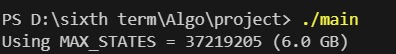
\includegraphics[width=0.5\textwidth]{images/figure_1.jpg}
    \captionof{figure}{Memory usage: \texttt{MAX\_STATES = 37,219,205} consuming \textbf{6.0 GB}}
\end{minipage}

\vspace{1em}

\noindent
\begin{minipage}{\textwidth}
    \centering
    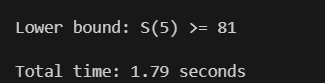
\includegraphics[width=0.4\textwidth]{images/gpu_based.png}
    \captionof{figure}{Execution output showing \textbf{Lower Bound: S(5) $\geq$ 81} with a runtime of \textbf{1.79 seconds}}
\end{minipage}

\subsection*{Drawbacks}
\begin{itemize}
    \item \textbf{Memory bottleneck:} Despite a powerful GPU, the number of states grew exponentially, capping at \( z = 81 \).
    \item \textbf{No pruning:} This brute-force method does not eliminate symmetries or exploit problem-specific heuristics.
    \item \textbf{Lack of scalability:} Moving to \( z > 81 \) would require more memory than the maximum available GPU memory or a fundamentally different approach.
\end{itemize}

\subsection*{Conclusion}
While this CUDA BFS implementation showcased impressive speed and parallelism, the exponential memory growth made it impractical for pushing Schur(5) much further. This motivated us to explore smarter strategies such as \textbf{Monte Carlo search}.


\newpage

\section{Optimized Approach: Hybrid Monte Carlo + GPU BFS}

\subsection*{Code Overview}
This implementation combines stochastic sampling on the CPU with parallel processing on the GPU:
\begin{itemize}
    \item \textbf{Step 1 (Monte Carlo Sampling):} Generates thousands of randomized, valid partial colorings up to $Z_0 = 20$ using the CPU.
    \item \textbf{Step 2 (GPU BFS):} Each valid prefix is used as a starting point for exhaustive GPU BFS from $z = 21$ onward.
\end{itemize}

\textbf{Result:} Successfully reached \textbf{$z = 113$}, surpassing the memory-limited BFS approach.

\subsection*{Code}
This implementation, \texttt{hybrid\_schur5.cu}, leverages both CPU and GPU strengths:
\begin{itemize}
    \item Uses \textbf{Monte Carlo rollouts} on the CPU to explore diverse partial colorings up to a depth of $Z_0 = 20$.
    \item Feeds successful rollouts into a \textbf{GPU-based breadth-first search}, significantly accelerating the search for higher $z$ values.
    \item Combines stochastic sampling and parallel expansion for efficient coverage of the search space.
\end{itemize}

\textbf{Advantages:}
\begin{itemize}
    \item \textbf{Scalability:} GPU threads process multiple states in parallel, allowing exploration of larger $z$ values.
    \item \textbf{Exploration diversity:} The Monte Carlo phase introduces randomness, increasing the chances of discovering fruitful initial states.
    \item \textbf{Memory efficiency:} The GPU rollout only continues from promising partial colorings, avoiding state explosion early on.
    \item \textbf{Performance:} Achieved a new milestone with \textbf{$z = 113$} while maintaining a manageable memory footprint.
\end{itemize}


\vspace{1em}

\noindent
\begin{minipage}{\textwidth}
    \centering
    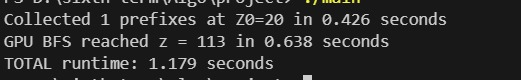
\includegraphics[width=0.5\textwidth]{images/figure_3.jpg}
    \captionof{figure}{Monte Carlo rollout phase collecting valid prefixes up to \texttt{Z\_0 = 113}.}
\end{minipage}









\newpage

\section{Comparison of Results}

\subsection*{Performance Summary}
\begin{tabular}{|l|c|c|}
\hline
Method & Max z Reached & Notes \\
\hline
Pure GPU BFS & 81 & Memory limit hit \\
Hybrid MC + BFS & 113 & Efficient prefix sampling \\
\hline
\end{tabular}

\subsection*{Observations}
\begin{itemize}
  \item The hybrid approach performs better because it prunes the search space early using randomness.
  \item The pure BFS approach scales poorly due to state explosion.
  \item Random rollouts up to a moderate $Z_0$ increase efficiency dramatically.
\end{itemize}

\section{Conclusion}

Using a hybrid approach combining CPU-based Monte Carlo sampling and GPU-based exhaustive search significantly increases the depth reachable in Schur number coloring problems. This method balances randomness and computation to overcome memory and complexity limitations.

\end{document}
